% INTRODUCTION

\chapter{Introduction}
\label{chap-Introduction}

\section{Motivation}

%Physical phenomena of turbulence
The turbulent phenomena that takes place in fluid flows is one of the most fascinating and, at the same time, challenging problems of classical physics. We can find examples of turbulent flows in many situations of our daily life, from the most known and noticeable like the jets leftover by airplanes in the sky or the flow of a river in the mountains, to the most inconspicuous like the turbulent flow that we generate in the morning cup of coffe. Another peculiarity that makes turbulent flows captivating is the wide range of scales in which it appears, starting from the astrophysics with the turbulent flows developed within the stars, to the turbulence that is observed in the biological cells flow.

Despite all the effords dedicated to understand the turbulent phenomena, this is a classical mathematical physics problem that still remains unsolved to this day. Many physists, mathematicians and engineers have been studying this problem during the 19th and 20th Centuries, and the prediction of turbulent behaviour with a certain degree of reliability is not completely understood yet. Then, apart from the practical utility of a deep understanding of its nature, the study of turbulence is also motivated by its inherent intellectual challenge.

It is said that there are two main motivations to study turbulence, physics and engineering. From the physics point of view, the nature of turbulence must be explored to understand the behaviour of such flows at al levels. On the other hand, from the engineering point of view, there are some problems that have to be solved and a solution to them must be given with the knowledge we have now, although it might be incomplete. As an engineering thesis, the motivation of this work relies on the engineering point of view. The approach will be to contribute in developing novel techniques for the simulation of incompressible turbulent flows, making use of the current knowlege of turbulent flow phenomena.

%CFD as a solution
Analytical solutions of fluid flows can only be obtained under certain restrictions and usually this restrictions can not be satisfied in real applications. Thus, we need other approaches to obtain the solution of a fluid flow different from the analytical description. The numerical solution is an alternative to determine the behaviour of fluid flows, which basically consists on approximate the solution defined over a continuous domain by a discrete solution defined in a finite set of points. This technique is known as Computational Fluid Dynamics (CFD) and it is widely used, both in the engineering and the physics worlds.

As it is depicted in the schematic diagram shown in \Fig{fig-CFD}, we can think that CFD leans on the intersection of three different topics: fluid mechanics, software engineering and physical applications. The fluid mechanics field give the basic knowledge of the physical phenomena that describes the fluid flow motion. The software engineering is needed to build codes able to simulate the fluid flow. Finally, we need the applications that give us the problem to be solved.

\begin{figure}[h!]
	\centering	
	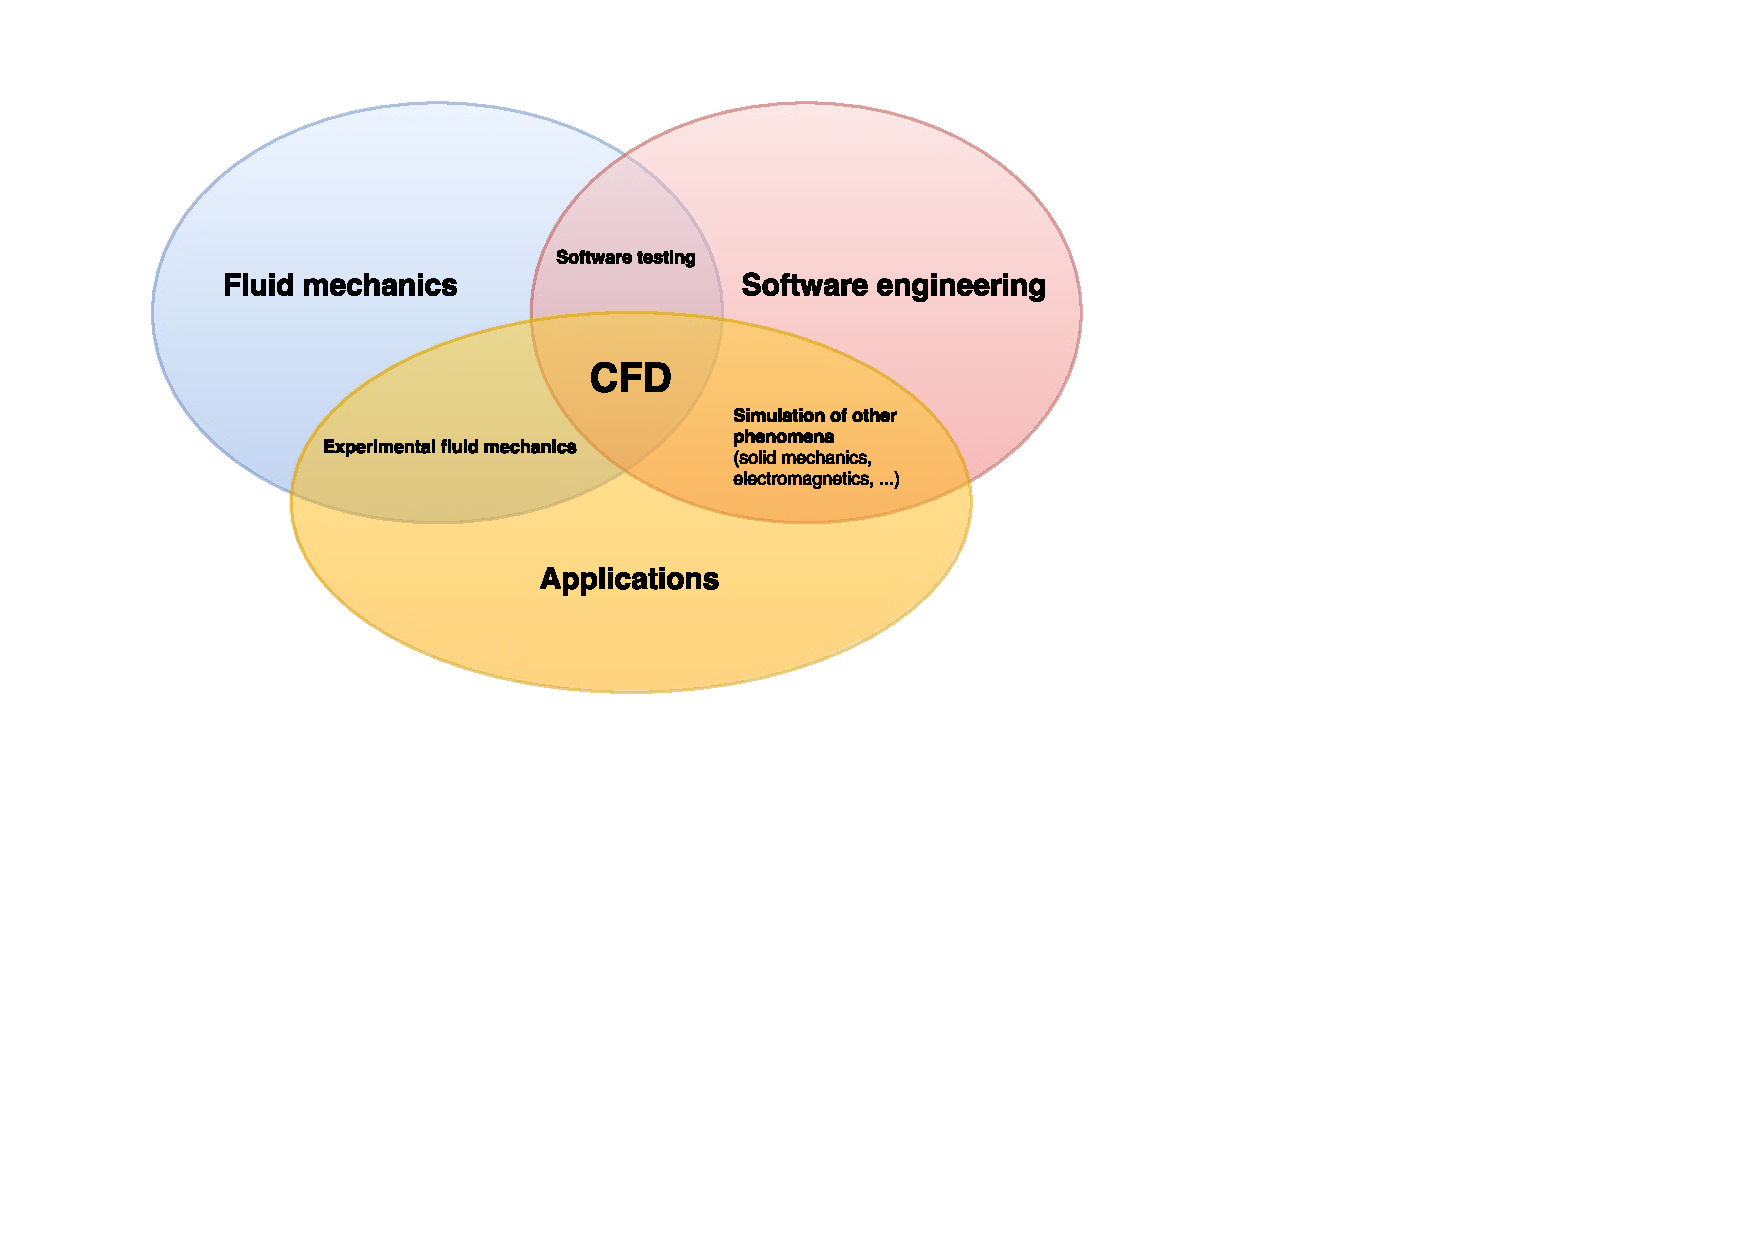
\includegraphics[trim=2cm 9cm 11cm 1cm,clip=true,width=0.7\textwidth]{Figures/Chapter1/CFD_scheme}
	\caption{Topics that conform CFD.}
	\label{fig-CFD}
\end{figure}

%Industrial problems
The CFD is widely used in many disciplines and industries like in the aerospace, automotive, chemical manufacturing, power generation, petroleum exploration, medical research, meteorology or astrophysics. It is a very valuable tool since it let to reductions in the cost of production by reducing the need of physical experimentation, improving the products or optimizing the production processes. In Table \ref{table-CFD_applications} we enumerate some more specific applications of CFD simulations that are very usefull for different disciplines.
\begin{table}[h]
\centering
\begin{tabular}{ll}
\toprule
Field&Application\\
\midrule
\midrule
\multirow{8}{*}{Biomedical}&Heart pumping\\
&Blood flow\\
&Air flow in lungs\\
&Nose and sinus flows\\
&Cell-fluid interface\\
&Artificial organ design\\
&Cardiac valve design\\
&Life support systems\\
\midrule
\multirow{1}{*}{Electronics}&Cooling flow in electronic devices\\
\midrule
\multirow{6}{*}{Aerospace and automotive}&Aerodynamic shape optimization\\
&Aerodynamic loads computation\\
&Turbines\\
&Propulsion systems\\
&Airbag Deployment\\
&In-Cylinder Engine Flow\\
\midrule
\multirow{4}{*}{Energy and power industry}&Heat exchange modeling\\
&Wind turbines blade design\\
&Pulverized coal combustion\\
&Emission of NOx particles\\
\midrule
\multirow{4}{*}{Environmental}&Impact of industrial exhausts\\
&Fire and smoke in buildings and tunnels\\
&Natural ventilation systems design\\
&Meteorology prediction\\
\midrule
\multirow{4}{*}{Civil}&Effect of wind on structures\\
&Water flow in rivers\\
&Water management\\
\bottomrule
\end{tabular}
\caption{CFD applications.}
\label{table-CFD_applications}
\end{table}

There already are CFD codes, both commercial and open source, that have the potential to solve a very broad spectrum of flow problems. However, the developement of computational algorithms for the simulation of turbulent flows is still an open topic. Moreover, the improvement of accuracy, the reduction of computational time and the increase of accessibility are also ongoing objectives in CFD. It is true that the CFD has some limitations, but the economic value of industrial applications has been demonstrated in a variety of industries.


FE methods as CFD

Exascale computing

Large scale solvers

Other applications 

COMFUS group


%From a technological point of view, nuclear fusion is considered as a safe and clean source of energy. In order to satisfy the future and increasing energetic needs of the society, there is the necessity  of efficient energy sources with a low $CO_2$ discharge. The increasing demand of energy sources that satisfy these conditions make nuclear fusion a strategic commitment for the EU energetic future.
%
%To make this energy source feasible, there must be a huge industrial development of the technology needed for its generation. The significance of the development of such technology arises with the creation of plans and European commissions such as the European Commission in the European Fusion Programme. This programme controls the construction and its subsequent experimentation of the experimental reactor ITER (International Thermonuclear Experimental Reactor). ITER will not be a completed fusion reactor, but it will allow to validate different concepts and technology needed to achieve the first fusion reactor able to provide energy efficiently, DEMO (DEMOnstration power plant). It is expected that ITER will be partially operative in 2017, but some tests such as the Tritium extraction will not be able to be performed until 2027. This date is too far given that the DEMO reactor is expected to be operative in the 2040 decade. This disadvantage explains the increasing need of numerical tools able to simulate the physical processes that occur in the nuclear fusion reactor. For instance, the European commission for the nuclear fusion development, Fusion for Energy (F4E), is opening constantly new calls for numerical investigations that allow the development of the needed technology. Currently, F4E is collaborating with the group where this thesis is being developed (COMFUS group) in different lines of research, all of them related with the Starting Grant project of the European Research Council (ERC) headed by professor Santiago Badia. 
%
%The objective of the COMFUS group is to develop significant advances on the simulation of the technology needed for the nuclear fusion. In this direction, the thesis is planed over the line of the development of numerical algorithms and computational tools able to simulate unsolved technological problems such as: 1) the plasma disruptions and magnetic confinement for large tokamaks and 2) the neutron shielding and the Tritium extraction inside the Test Blanket Modules (TBM). 

\section{Thesis objectives}

The TBMs that wrap the fusion reactor core are a fundamental part of it. These modules not only are the responsible of the shielding that absorb the neutrons that emerge from the plasma, but also are the place where the Tritium is extracted. Tritium is needed to keep the plasma and it can not be found in nature, so its extraction is a key step. One of its design consists on a micro-channel system full of  liquid metal. Because of the magnetic forces that confine the plasma inside the reactor core, this liquid is subjected to the magnetohydrodynamics (MHD) equations.

As said before, these components can not be tested in ITER before 2027. When this occurs, its configuration will not be the same that the needed for the DEMO reactor. Then, the tests done in ITER reactor will mainly be used as a validation of the numerical simulation codes that will be used in the final design of the TBMs for the DEMO reactor.

These conditioning aspects imply that the research on numerical simulations able to reproduce such processes are a key step in the development of the nuclear fusion energy. In this thesis project we will continue the work of the COMFUS group in this line.

The liquid metals are electrical conductors that are subjected to the MHD physical laws, which couple the Navier-Stokes equations with Maxwell equations. These flows have a particular behaviour due to the magnetic effects. For a low magnetic Reynolds, the energy spectra is different of the defined by the classical flow theory. For this reason, it is necessary to \emph{develop numerical models able to simulate the quasi2D turbulence} that appears in these processes.

The stabilized finite element formulation for incompressible MHD, tested in laminar regime, that will be used in this thesis has been proposed recently by the group where this thesis is developed. The main novelty with respect to existent formulations is the use of the same interpolation for the fluid-dynamic and magnetic problems, keeping the optimal convergence. At this point, we want to explore its extension to turbulent cases by the use of Variational MultiScale (VMS) methods. These methods arise as a numerical stabilization techniques, but also model successfully the classical flow turbulence since they introduce numerical dissipation efficiently. Therefore, we firstly will \emph{test these methods in classical turbulent flows} to verify their applicability to a more complex turbulent flows. From this point, we want to apply the same methods to simulate the liquid metal problem, which is influenced by the magnetic field, and reproduce accurately the quasi2D turbulence.

The applications we have in mind are extremely complex and require large computational resources. The largest supercomputers are distributed-memory machines with thousands of cores. It is a very hard task to efficiently run simulation codes on these platforms. It requires excellent implementations and robust solvers, based on efficient preconditioners and Krylov solvers. The COMFUS team is actively working in this area, and the FEMPAR code developed by the team has already proved excellent scalability results up to 30,000 cores. The solvers used by the team combine robust and scalable solvers for symmetric positive definite problems and block-preconditioning. This approach allows to deal with indefinite problems like the Stokes system and fluids at low Reynolds numbers. However, there is still the challenge to scale up nonsymmetric and indefinite problems. In order to do so, we are forced to implement and \emph{develop novel techniques for nonsymmetric problems}.

The team has been actively working on new block preconditioners for inductionless and resistive MHD systems. These preconditioners, based on inexact-block LU factorizations, are used in combination with Krylov methods. Since these preconditioners are computationally intensive, it would be very appealing to use them as solvers instead of preconditioners. This approach, in the frame of resistive MHD has been exploited in \cite{badia_unconditionally_2012}, where the $\theta$ scheme was used for time integration. We plan to develop novel operator splitting methods based on implicit-explicit Runge-Kutta schemes. In particular, we want to \emph{design schemes that split velocity-pressure computations}.

Finally and related to the use of VMS methods, we want to \emph{test the advantages of the symmetric projection stabilization methods} with respect to classical VMS formulations.
%Besides to use these block preconditioners to solve the multiphysic problems, this thesis proposal also expect to use the block preconditioners structure to develop new time integrators which decouples the different physical problem variables. The idea is to take advantage of the Implicit-Explicit (IMEX) time integration technique using a Runge-Kutta scheme and operate with the different blocks to decouple the different physical fields that appears into the problem.
%
%\subsection{Large scale computation}
%As it has been said before, the physical processes that takes place in a nuclear fusion reactor lead to complex systems of equations. Besides the coupling between different physical problems, there also appear several length and time scales, resulting in a multi-scale problems. The way to solve accurately problems with large time scales without having numerical inestabilities and without using a small really time step, is by implicit methods. However, these methods require to solve nonlinear systems at each time-step. Then, there arise the need to use scalable solvers for massivelly parallel computers.
%
%It has to be said that the COMFUS group has an extensive experience in this topic. The code that will be used by the thesis development is designed to be used in distributed computers and it incorporates domain decomposition (DD) methods optimal for large scale problems that can be combined in a natural way with block preconditioners. The scalability of these methods has been proved to be excellent until 4096 CPUs {\color{red}(o mes??)}.
%
%To this end, this thesis project considers:
%\begin{itemize}
%\item {\bf Block preconditioners implementation and computational aspects}. As was said before, the multiphysical problem can be rewritten as a block system, i. e., one block for each unknown of the global problem. The non-diagonal blocks are those which couples the different subproblems. Here, the key decision is how to reorganize the system and subsequently how to define a good approximation to the original matrix, which will be used as a preconditioner. These preconditioners must be spectrally equivalent to the original matrix of the system of equations.
%
%{\color{red}... (Santi, queda alguna cosa a fer en aquest apartat? Em sembla que tot el que vam posar a la proposta de la FPU es lo que ja heu fet amb l'Alberto i el Ramon)}
%
%\item {\bf Domain Decomposition solvers for convection dominated flows}. {\color{red} ... (Aquest apartat no hi era a la proposta FPU, però l'he posat per mencionar lo del BDDC. Alguna idea per posar aqui?)}
%\end{itemize}

\section{Document structure}
